\chapter{From Maxwell to Coupled Modes}
\label{ch:maxwell-coupled-modes}

\begin{chapterlead}
Much of non-Hermitian photonics is discussed in the language of $2\times 2$
matrices: two coupled resonances, an exceptional point where eigenvalues
coalesce, a $\PT$-symmetric Hamiltonian with balanced gain and loss.
Where do these finite-dimensional matrices come from? This chapter
answers that question by deriving coupled-mode models as controlled
reductions of the full Maxwell eigenproblem. The derivation makes
explicit what is gained and what is lost in the reduction, and establishes
the conditions under which a non-Hermitian effective Hamiltonian
faithfully represents the physics of the underlying electromagnetic system.
\end{chapterlead}


%% ================================================================
\section{Three levels of description}
\label{sec:three-levels}

Before proceeding with derivations, it is important to distinguish three
levels of electromagnetic description that are often conflated in the
literature:

\begin{enumerate}
 \item \textbf{The full Maxwell operator.} The infinite-dimensional
 operator $\Mop$ or its first-order form $\hat{\mathcal{M}}$, acting
 on the complete space of electromagnetic fields. Self-adjoint for
 lossless closed systems; non-self-adjoint when any of the three
 conditions of Chapter~\ref{ch:energy-inner} is violated.

 \item \textbf{The complete modal expansion.} A representation of the
 field as a sum over \emph{all} eigenmodes (normal modes, QNMs,
 radiation modes). This is formally exact but impractical: the sum
 involves infinitely many modes and, for open systems, the continuous
 spectrum.

 \item \textbf{The truncated effective Hamiltonian.} A finite-dimensional
 matrix $H_{\mathrm{eff}}$ acting on a small number of retained modes.
 This is the object that appears in most coupled-mode analyses.
 It is generically non-Hermitian, even when the full Maxwell operator
 is self-adjoint, because the discarded modes act as an environment.
\end{enumerate}

The passage from level~1 to level~3 is a projection. The non-Hermiticity
of $H_{\mathrm{eff}}$ arises from the projection as much as from any
intrinsic non-Hermiticity of the material or boundary conditions. This
is the fourth road to non-Hermiticity identified in
Section~\ref{ssec:road-projection}.


%% ================================================================
\section{Temporal coupled-mode theory}
\label{sec:tcmt}

\subsection{The phenomenological starting point}
\label{ssec:tcmt-phenom}

Temporal coupled-mode theory (TCMT), as introduced by Haus and later
systematized by Fan and collaborators~\cite{v2024exact,zhao2019connection}, models a set of $N$ resonant modes
coupled to $M$ input--output channels. The dynamics of the mode amplitudes
$\mathbf{a}(t) = (a_1, \ldots, a_N)^\transpose$ are governed by
\begin{equation}
 \dv{\mathbf{a}}{t}
 = \bigl(-i\boldsymbol{\Omega} - \boldsymbol{\Gamma}\bigr)\,\mathbf{a}
 + \mathbf{K}^\transpose\,\mathbf{s}_+,
 \label{eq:tcmt-time}
\end{equation}
where $\boldsymbol{\Omega}$ is the Hermitian frequency matrix,
$\boldsymbol{\Gamma}$ is the (positive semi-definite) decay-rate matrix,
$\mathbf{K}$ is the coupling matrix between modes and channels, and
$\mathbf{s}_+$ is the vector of incoming wave amplitudes. The outgoing
waves are
\begin{equation}
 \mathbf{s}_- = \mathbf{C}\,\mathbf{s}_+
 + \mathbf{K}\,\mathbf{a},
 \label{eq:tcmt-output}
\end{equation}
where $\mathbf{C}$ is the direct scattering (background) matrix.

The effective Hamiltonian is
\begin{equation}
 H_{\mathrm{eff}} = \boldsymbol{\Omega} - i\boldsymbol{\Gamma},
 \label{eq:heff-tcmt}
\end{equation}
which is manifestly non-Hermitian whenever $\boldsymbol{\Gamma} \neq 0$
(i.e., whenever the resonances have finite lifetime). The eigenvalues of
$H_{\mathrm{eff}}$ are the complex resonance frequencies $\omtil_n$; they
coincide with the QNM frequencies of the open system when the model is
accurate.

\subsection{TCMT constraints from energy conservation}
\label{ssec:tcmt-constraints}

Energy conservation and time-reversal symmetry impose algebraic
constraints on the TCMT parameters. For a lossless system with
reciprocal coupling:
\begin{align}
 \boldsymbol{\Gamma} &= \frac{1}{2}\mathbf{K}^\dagger\mathbf{K},
 \label{eq:tcmt-gamma}\\
 \mathbf{C}\mathbf{K}^* &= -\mathbf{K},
 \label{eq:tcmt-ck}
\end{align}
which together ensure that $\Smat(\omega)$ is unitary on the real axis
when material losses are absent. These constraints reduce the number of
free parameters in the TCMT model and provide self-consistency checks.

\paragraph{Derivation from energy balance.}
Constraint~\eqref{eq:tcmt-gamma} follows from requiring that the total
stored energy $W = \mathbf{a}^\dagger\mathbf{a}$ decays at a rate equal
to the total power emitted into all channels. From~\eqref{eq:tcmt-time}
with $\mathbf{s}_+ = 0$ (no input), the energy decay rate is
\begin{equation}
 \dv{W}{t} = \mathbf{a}^\dagger\dv{\mathbf{a}}{t}
 + \biggl(\dv{\mathbf{a}}{t}\biggr)^{\!\dagger}\mathbf{a}
 = -2\,\mathbf{a}^\dagger\boldsymbol{\Gamma}\,\mathbf{a}.
 \label{eq:energy-decay-rate}
\end{equation}
The power emitted into channels is
$P_{\mathrm{out}} = \mathbf{s}_-^\dagger\mathbf{s}_-
= \mathbf{a}^\dagger\mathbf{K}^\dagger\mathbf{K}\,\mathbf{a}$
(using $\mathbf{s}_+ = 0$ in~\eqref{eq:tcmt-output}).
Equating $|\dd W/\dd t| = P_{\mathrm{out}}$ for arbitrary
$\mathbf{a}$ yields~\eqref{eq:tcmt-gamma}.

Constraint~\eqref{eq:tcmt-ck} follows from time-reversal symmetry:
the time-reversed outgoing field must be a valid incoming field that
excites the time-reversed mode amplitudes. In the frequency domain,
this requires $\Smat(\omega)\Smat^*(\omega) = \mathbf{I}$ on the real
axis, which, after expanding $\Smat$ in terms of
$H_{\mathrm{eff}}$, reduces to~\eqref{eq:tcmt-ck}.

For a system with material loss or gain, the constraints are modified:
$\boldsymbol{\Gamma}$ acquires additional contributions from intrinsic
loss rates, and unitarity is replaced by a weaker bound
$\Smat^\dagger\Smat \le \mathbf{I}$ (for passive systems).

\subsection{What TCMT does not tell us}
\label{ssec:tcmt-limitations}

Equations~\eqref{eq:tcmt-time}--\eqref{eq:tcmt-output} are
phenomenological~\cite{icon2022imaginary,alpeggiani2017quasinormal,opg2021non}: they postulate a finite-dimensional linear system and
constrain its parameters by energy conservation and time-reversal
symmetry. They do not derive $\boldsymbol{\Omega}$,
$\boldsymbol{\Gamma}$, or $\mathbf{K}$ from the electromagnetic fields.
Nor do they specify which modes should be retained or how the truncation
error scales.

A Maxwell-first monograph must go further: it must connect the TCMT
parameters to the spatial field distributions and material properties of
the photonic structure. This is what the QNM-based derivation provides.


%% ================================================================
\section{Deriving the effective Hamiltonian from QNMs}
\label{sec:heff-derivation}

\subsection{Starting point: the QNM expansion}
\label{ssec:qnm-start}

Consider a photonic structure supporting $N$ well-separated QNMs
$\{\tilde{\EE}_n\}$ with complex frequencies $\{\omtil_n\}$, normalized
according to the unconjugated prescription of
Section~\ref{sec:qnm-normalization}. The Green tensor near the
resonances is (from~\eqref{eq:green-qnm})
\begin{equation}
 \mathbf{G}(\rr,\rr';\omega)
 \approx \sum_{n=1}^{N}
 \frac{c^2\,\tilde{\EE}_n(\rr)\otimes\tilde{\EE}_n(\rr')}
 {2\omtil_n(\omega - \omtil_n)}.
 \label{eq:green-few-mode}
\end{equation}

\subsection{Mode amplitudes and equations of motion}
\label{ssec:mode-amplitudes}

Expand the electric field in the vicinity of the resonator as
\begin{equation}
 \EE(\rr,t) = \sum_{n=1}^{N} a_n(t)\,\tilde{\EE}_n(\rr)
 + \EE_{\mathrm{rad}}(\rr,t),
 \label{eq:field-expansion}
\end{equation}
where $a_n(t)$ are time-dependent mode amplitudes and
$\EE_{\mathrm{rad}}$ is the contribution from the radiation continuum and
distant modes. Projecting the time-domain Maxwell equations onto the
QNM basis using the biorthogonal inner product yields, after neglecting
the continuum coupling and assuming slowly varying amplitudes,
\begin{equation}
 \dv{a_n}{t} = -i\omtil_n\,a_n - i\sum_{m\neq n} V_{nm}\,a_m
 + f_n(t),
 \label{eq:eom-amplitudes}
\end{equation}
where $V_{nm}$ is the coupling between QNMs $n$ and $m$ induced by any
perturbation (e.g., a nearby scatterer or a change in $\epsr$), and
$f_n(t)$ represents the driving by external sources.

\subsection{Mode-overlap integrals}
\label{ssec:mode-overlap}

The coupling matrix elements $V_{nm}$ are determined by mode-overlap
integrals. For a permittivity perturbation $\delta\epsr(\rr)$
(e.g., bringing two cavities into proximity), the coupling is
\begin{equation}
 V_{nm} = -\frac{\omtil_n}{2}
 \int \delta\epsr(\rr)\,\tilde{\EE}_n(\rr)\cdot\tilde{\EE}_m(\rr)
 \;\dd^3r,
 \label{eq:coupling-overlap}
\end{equation}
where the integral is over the region where $\delta\epsr \neq 0$.
This formula connects the abstract matrix element to a spatial integral
of the electromagnetic fields and the material perturbation: placing the
perturbation where both mode fields are strong maximizes the coupling.

For a reciprocal medium, Lorentz reciprocity makes the properly
normalized first-order coupling matrix complex symmetric, but not
Hermitian. Equation~\eqref{eq:coupling-overlap} is a compact scalar
perturbation formula; when the frequencies of the two modes differ
substantially, the prefactor and normalization must be treated with care.
Near a degenerate pair it is common to use a symmetrized reference
frequency, giving $V_{nm}=V_{mn}$ to the same perturbative order. The
important point is that reciprocity implies transpose symmetry, not
complex-conjugate symmetry.

\subsection{The effective Hamiltonian}
\label{ssec:heff-matrix}

In matrix form, the homogeneous part of~\eqref{eq:eom-amplitudes} is
\begin{equation}
 i\,\dv{\mathbf{a}}{t} = H_{\mathrm{eff}}\,\mathbf{a},
 \qquad
 (H_{\mathrm{eff}})_{nm} = \omtil_n\,\delta_{nm} + V_{nm}.
 \label{eq:heff-matrix}
\end{equation}
This is a non-Hermitian matrix whose diagonal entries are the complex QNM
frequencies and whose off-diagonal entries are the inter-mode couplings.
It is the Maxwell-derived counterpart of the phenomenological
$H_{\mathrm{eff}} = \boldsymbol{\Omega} - i\boldsymbol{\Gamma}$ from
TCMT, with the crucial advantage that every matrix element is determined
by the electromagnetic fields and material properties.

\begin{takeaway}[From Maxwell to matrix]
The non-Hermitian effective Hamiltonian of coupled-mode theory is not a
postulate---it is a controlled approximation to the full Maxwell
eigenproblem, obtained by expanding in QNMs and projecting out the
radiation continuum. Its non-Hermiticity has two sources: the intrinsic
complex frequencies of the QNMs (from radiation or absorption) and the
truncation of the modal basis.
\end{takeaway}


%% ================================================================
\section{Example: two coupled cavities}
\label{sec:two-cavity-example}

Consider two identical photonic crystal cavities, each supporting a
single QNM at complex frequency $\omtil_0 = \omega_0 - i\gamma_0$,
separated by a barrier of $N_b$ lattice periods.

\subsection{Isolated-cavity QNMs}
\label{ssec:isolated-cavities}

Each isolated cavity has a QNM field $\tilde{\EE}_0(\rr)$ that decays
evanescently into the barrier as $\exp(-\kappa_{\mathrm{gap}}x)$, with
characteristic length $\ell_{\mathrm{ev}} = 1/\kappa_{\mathrm{gap}}$.
Here $\kappa_{\mathrm{gap}}$ is the evanescent decay constant at the gap
frequency and $a$ is the lattice period.

When the cavities are brought to a separation $d = N_b a$, the field
of cavity~1 has a small but nonzero amplitude at the location of
cavity~2, and vice versa. The perturbation is the presence of the
other cavity, described by $\delta\epsr(\rr)$ in the region of
cavity~2.

\subsection{Coupling strength}
\label{ssec:coupling-strength}

The coupling matrix element~\eqref{eq:coupling-overlap} gives
\begin{equation}
 V_{12} = -\frac{\omtil_0}{2}
 \int_{\mathrm{cav\,2}} \delta\epsr(\rr)\,
 \tilde{\EE}_1(\rr)\cdot\tilde{\EE}_2(\rr)\;\dd^3r
 \approx \kappa_0\,e^{-\kappa_{\mathrm{gap}} d},
 \label{eq:two-cavity-coupling}
\end{equation}
where $\kappa_0$ is a prefactor determined by the QNM field profiles and
the dielectric contrast. The exponential dependence on the
barrier thickness $d$ is the signature of evanescent coupling.

For a typical silicon photonic crystal cavity at $\lambda = 1550\;\mathrm{nm}$
with $Q_0 = 10^4$ and $N_b = 3$ barrier periods, the coupling can be
$\kappa \sim 10^{11}\;\mathrm{rad/s}$, much larger than the decay rate
$\gamma_0 = \omega_0/(2Q_0) \sim 6 \times 10^{10}\;\mathrm{rad/s}$. In
this regime, the modes hybridize strongly, producing a symmetric and an
antisymmetric supermode with frequency splitting $2\kappa$.

\paragraph{Quantitative example.}
For concreteness, take a one-dimensional photonic crystal of GaAs
($\varepsilon = 12.25$) and air with period $a = 350\;$nm, supporting
a defect cavity at $\lambda_0 = 1550\;$nm with $Q_0 = 8000$. Then
$\omega_0 = 2\pi c/\lambda_0 \approx 1.215 \times 10^{15}\;$rad/s,
$\gamma_0 = \omega_0/(2Q_0) \approx 7.6 \times 10^{10}\;$rad/s.
With $N_b = 4$ barrier periods and an evanescent decay constant
$\kappa_{\mathrm{gap}}\,a \approx 1.2$, the inter-cavity coupling is
$\kappa \approx \kappa_0\,e^{-4 \times 1.2} \approx 8.3 \times 10^{-3}\,\kappa_0$.
For $\kappa_0 \sim 5 \times 10^{13}\;$rad/s (estimated from the
mode-overlap integral), this gives
$\kappa \approx 4.2 \times 10^{11}\;$rad/s, so
$\kappa/\gamma_0 \approx 5.5$: the system is in the strong-coupling
regime. The supermode splitting is $2\kappa \approx 8.4 \times
10^{11}\;$rad/s, corresponding to a wavelength splitting
$\Delta\lambda \approx \lambda_0^2\,\kappa/(\pi c) \approx 1.1\;$nm.
This splitting is easily resolvable in a standard optical spectrum
analyser, confirming that the two-mode Hamiltonian makes a testable
prediction.

Reducing the barrier to $N_b = 2$ increases $\kappa$ by a factor
$e^{2 \times 1.2} \approx 11$, bringing $\kappa/\gamma_0 \approx 60$:
the modes are deeply hybridized and the splitting dominates the
linewidth. Increasing the barrier to $N_b = 6$ reduces $\kappa$ below
$\gamma_0$, placing the system in the weak-coupling regime where the
supermode splitting is unresolved and the two resonances merge into a
single broadened peak.

\subsection{The two-mode Hamiltonian}
\label{ssec:two-mode-hamiltonian}

The effective Hamiltonian for the two-cavity system is
\begin{equation}
 H_{\mathrm{eff}} = \begin{pmatrix}
 \omtil_0 & V_{12} \\
 V_{21} & \omtil_0
 \end{pmatrix}
 = \omega_0 \mathbf{I} - i\gamma_0 \mathbf{I}
 + \begin{pmatrix} 0 & \kappa \\ \kappa & 0 \end{pmatrix},
 \label{eq:two-cavity-heff}
\end{equation}
where $\kappa = V_{12} = V_{21}$ (reciprocity) and $\kappa$ is real to
lowest order in the evanescent overlap. The eigenvalues are
$\omtil_\pm = \omega_0 - i\gamma_0 \pm \kappa$: two real-split modes
with the same decay rate.

If the two cavities are made non-identical---one with additional gain
and the other with additional loss---the diagonal entries become
$\omtil_0 \pm i\gamma_{\mathrm{gl}}$, and the Hamiltonian is the
$\PT$-symmetric model of Chapter~\ref{ch:pt-symmetric} with a
Maxwell-derived coupling $\kappa$.

\begin{figure}[t]
 \centering
 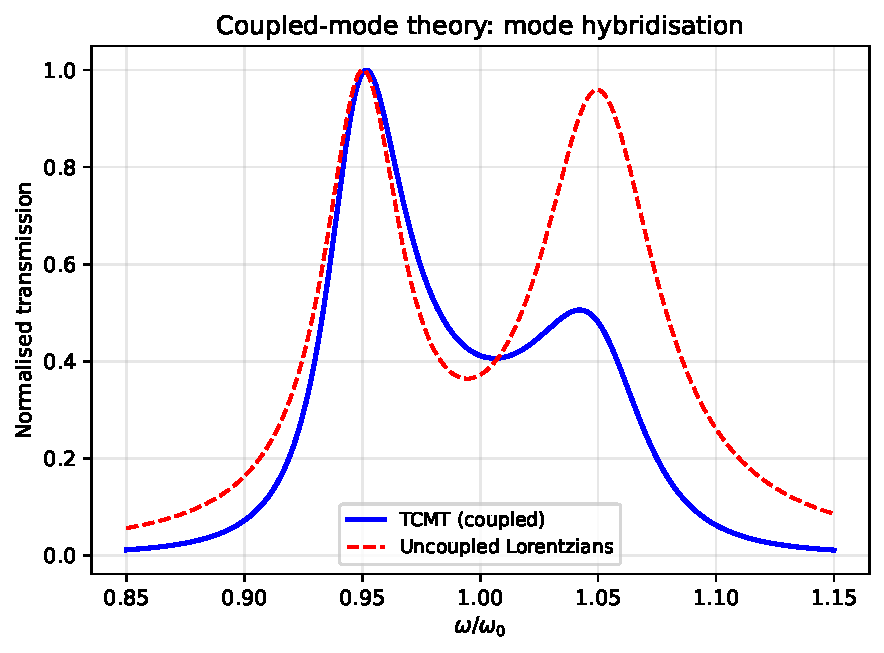
\includegraphics[width=0.68\linewidth]{figures/fig_f07_reaction_cmt.pdf}
 \caption{Coupled-mode hybridisation in a two-resonator system. The
 TCMT prediction (blue) shows the splitting produced by coherent
 inter-cavity coupling, while the uncoupled Lorentzian estimate (red
 dashed) misses the hybridised supermodes. The comparison emphasizes
 why the reaction and QNM-overlap derivations are needed: coupling is
 not a phenomenological fitting parameter but a Maxwell overlap integral
 between open resonator fields.}
 \label{fig:reaction-cmt}
\end{figure}


%% ================================================================
\section{The reaction inner product}
\label{sec:reaction}

An alternative derivation of coupled-mode equations, developed by Xu and
Chen~\cite{xu2015general}, uses the concept of \emph{reaction} from
electromagnetic theory. The reaction of a field $(\EE_a, \HH_a)$ on a
source $\JJ_b$ is
\begin{equation}
 \langle a, b\rangle_{\mathrm{R}}
 = \int \EE_a\cdot\JJ_b\;\dd^3 r,
 \label{eq:reaction-def}
\end{equation}
which is an unconjugated bilinear form---the same structure as the QNM
normalization of Section~\ref{sec:qnm-normalization}.

\subsection{Reciprocity and the symmetric coupling}
\label{ssec:reaction-reciprocity}

For a reciprocal medium, the Lorentz reciprocity theorem
(Section~\ref{sec:reciprocity}) ensures that
$\langle a, b\rangle_{\mathrm{R}} = \langle b, a\rangle_{\mathrm{R}}$:
the reaction is symmetric. This symmetry is the foundation for a
\emph{generalized coupled-mode theory} (GCMT) that works in non-Hermitian
waveguides, where the standard power-conservation-based CMT
fails~\cite{xu2015general}.

The GCMT replaces the Hermitian power inner product
$\langle\EE_a^*,\EE_b\rangle$ with the reaction inner product
$\langle\EE_a,\EE_b\rangle_{\mathrm{R}}$ (no conjugation), and derives
coupled-mode equations that remain valid even in $\PT$-symmetric and
gain--loss waveguides. The resulting coupling matrix is symmetric
(by reciprocity) but not Hermitian---precisely the structure expected for
a non-Hermitian system that is still reciprocal.

\subsection{Connection to QNM biorthogonality}
\label{ssec:reaction-qnm}

The reaction inner product and the QNM biorthogonal inner product are
closely related. For two QNMs of the same structure, the biorthogonality
relation~\eqref{eq:biorthogonality} can be rewritten as a vanishing
reaction:
\begin{equation}
 \langle\tilde{\EE}_m,\,\epsr\tilde{\EE}_n\rangle_{\mathrm{R}}
 = \int \epsr(\rr)\,\tilde{\EE}_m(\rr)\cdot\tilde{\EE}_n(\rr)\;\dd^3r
 = 0
 \qquad (m \neq n).
 \label{eq:reaction-biorthogonal}
\end{equation}
This confirms that the QNM-based and reaction-based derivations of
coupled-mode theory are different presentations of the same underlying
structure: both use unconjugated bilinear forms enforced by reciprocity.

\subsection{When reaction-CMT and TCMT disagree}
\label{ssec:reaction-tcmt-disagree}

For Hermitian waveguides, the reaction inner product and the standard
power-orthogonality inner product give equivalent coupled-mode
equations. However, for non-Hermitian waveguides with gain or loss,
the two approaches can give \emph{different} coupling coefficients.
The standard power-based CMT assumes $\langle\EE_a^*,\EE_b\rangle$ is
the correct overlap, which is valid only when the modes carry positive
definite power. In a gain--loss waveguide, some modes can carry
negative power (the field does work on the medium rather than the
reverse), and the power-orthogonality assumption fails.

The reaction-based CMT avoids this problem because the reaction inner
product does not involve complex conjugation and does not require
positive definiteness. It is therefore the correct starting point for
deriving coupled-mode equations in $\PT$-symmetric waveguides, gain
waveguides, and any system where the modes are not power-orthogonal.

The practical consequence is that the reaction-CMT coupling coefficient
between a gain mode and a loss mode can be purely imaginary, even when
the waveguides are identical except for the sign of the imaginary part
of $\varepsilon$. This imaginary coupling is responsible for the
$\PT$ phase transition in coupled waveguides: below the transition
the coupling compensates the gain--loss imbalance, and above it the
eigenvalues become complex conjugate pairs.


%% ================================================================
\section{Two coupled resonances: the minimal model}
\label{sec:two-mode}

The simplest and most frequently used non-Hermitian model in photonics
is a pair of coupled resonances described by the $2\times 2$ matrix
\begin{equation}
 H_{\mathrm{eff}} =
 \begin{pmatrix}
 \omega_1 - i\gamma_1 & \kappa \\
 \kappa & \omega_2 - i\gamma_2
 \end{pmatrix},
 \label{eq:two-mode-H}
\end{equation}
where $\omega_j$ are the bare resonant frequencies, $\gamma_j$ the decay
rates, and $\kappa$ the coupling strength (real for a reciprocal system
without radiation coupling corrections).

The eigenvalues are
\begin{equation}
 \omtil_\pm = \bar{\omega} - i\bar{\gamma}
 \pm \sqrt{\left(\frac{\Delta\omega - i\Delta\gamma}{2}\right)^2
 + \kappa^2},
 \label{eq:two-mode-evals}
\end{equation}
where $\bar{\omega} = (\omega_1+\omega_2)/2$,
$\bar{\gamma} = (\gamma_1+\gamma_2)/2$,
$\Delta\omega = \omega_1 - \omega_2$, and
$\Delta\gamma = \gamma_1 - \gamma_2$.

When $\Delta\omega = 0$ (degenerate bare frequencies), the eigenvalues
become
\begin{equation}
 \omtil_\pm = \bar{\omega} - i\bar{\gamma}
 \pm \sqrt{\kappa^2 - \left(\frac{\Delta\gamma}{2}\right)^2}.
 \label{eq:two-mode-ep}
\end{equation}
An \emph{exceptional point} occurs when the square root vanishes:
$\kappa = |\Delta\gamma|/2$. At this point, not only the eigenvalues but
also the eigenvectors coalesce, and the matrix becomes defective (its
Jordan normal form contains a $2\times 2$ Jordan block). This is the
subject of Chapter~\ref{ch:exceptional-points}.


%% ================================================================
\section{Validity and breakdown}
\label{sec:cmt-validity}

The effective Hamiltonian~\eqref{eq:heff-matrix} is a useful and often
accurate model, but it is an approximation. Its validity requires:

\begin{enumerate}
 \item \textbf{Mode isolation.} The retained QNMs must be spectrally
 well separated from all other resonances and from the continuum
 threshold. Overlapping resonances require more modes or a different
 approach.

 \item \textbf{Weak perturbation.} The coupling $V_{nm}$ should be
 small compared to the frequency separation between modes, so that the
 perturbative projection is accurate.

 \item \textbf{Narrow bandwidth.} The driving field should have a
 bandwidth smaller than the free spectral range, so that only the
 retained modes are significantly excited.

 \item \textbf{Linearity.} The expansion assumes linear media. Near
 and above the lasing threshold, gain saturation introduces nonlinear
 corrections that are not captured by a linear $H_{\mathrm{eff}}$.
\end{enumerate}

When these conditions break down, the effective Hamiltonian picture fails
and one must return to the full Maxwell operator---either numerically or
through a more complete modal expansion. The practical question is not
whether a truncated model is ever exact, but whether the neglected modes
are far enough away that their effect can be treated perturbatively. A
clean way to express this is the Schur complement: partition the complete
modal Hamiltonian into retained modes $P$ and eliminated modes $Q$,
\begin{equation}
 H = \begin{pmatrix} H_{PP} & H_{PQ} \\
 H_{QP} & H_{QQ} \end{pmatrix}.
 \label{eq:schur-partition}
\end{equation}
Eliminating the $Q$ subspace gives the frequency-dependent effective
operator
\begin{equation}
 H_{\mathrm{eff}}(\omega)
 = H_{PP} + H_{PQ}\,(\omega - H_{QQ})^{-1}H_{QP}.
 \label{eq:schur-heff}
\end{equation}
The naive truncation keeps only $H_{PP}$. It is accurate only when
$\|H_{PQ}\|^2/\Delta$ is small, where $\Delta$ is the spectral separation
between the retained and eliminated modes. The Schur-complement
correction is second-order in $H_{PQ}$ and first-order in $1/\Delta$:
it systematically improves the naive truncation by accounting for the
virtual excitation of the eliminated modes.  The truncation is accurate
when the coupling-to-detuning ratio $\|H_{PQ}\|/\Delta$ is small;
the leading correction scales as $\|H_{PQ}\|^2/\Delta$.

\paragraph{Convergence with spectral separation.}
For the four-mode test model used in Figure~\ref{fig:qnm-cmt-truncation},
the naive two-mode truncation error (the maximum eigenvalue error
relative to the four-mode reference) is $\sim 1.1 \times 10^{-2}$ when
the eliminated modes are $5\gamma$ away, and decreases to
$\sim 8.5 \times 10^{-4}$ at $10\gamma$ separation. Including the
Schur-complement correction reduces these errors to
$\sim 4.8 \times 10^{-3}$ and $\sim 5.9 \times 10^{-5}$, respectively.
The leading Schur correction scales as $\|H_{PQ}\|^2/\Delta$,
so the residual error after correction is of order
$\|H_{PQ}\|^3/\Delta^2$---one power higher than the naive
truncation error.  This is why the green curves in
Figure~\ref{fig:qnm-cmt-truncation} converge much faster with
increasing spectral separation.

The practical lesson is clear: a two-mode model is adequate when the
nearest unretained resonance is more than $\sim 10$ linewidths away.
For denser spectra, more modes must be retained or the Schur complement
must be applied. This criterion directly impacts the design of
non-Hermitian photonic devices: a PT-symmetric laser operating near
an exceptional point is sensitive to distant modes precisely when the
Schur-complement correction becomes large.

\paragraph{Example: three-mode reduction to a two-mode
$\PT$-symmetric Hamiltonian.}
Consider three QNMs with complex frequencies
$\tilde{\omega}_1 = \omega_0 + i\gamma$,
$\tilde{\omega}_2 = \omega_0 - i\gamma$, and
$\tilde{\omega}_3 = \omega_0 + \Delta - i\gamma_3$, where
$\Delta \gg \gamma, \gamma_3$ is the detuning of the third mode from the
near-degenerate pair. Modes~1 and~2 form a gain--loss pair (balanced
when their real frequencies coincide and their imaginary parts are
opposite), while mode~3 is a distant lossy resonance. The
full $3\times 3$ Hamiltonian is
\begin{equation}
 H = \begin{pmatrix}
 \omega_0 + i\gamma & \kappa_{12} & \kappa_{13} \\
 \kappa_{12} & \omega_0 - i\gamma & \kappa_{23} \\
 \kappa_{13} & \kappa_{23} & \omega_0 + \Delta - i\gamma_3
 \end{pmatrix},
 \label{eq:three-mode-full}
\end{equation}
where $\kappa_{ij}$ are inter-mode couplings from the reaction inner
product~\eqref{eq:reaction-def}; in this example they are taken real,
so the matrix is real-symmetric apart from the diagonal gain/loss
terms.  We treat modes~1 and~2 as the
retained subspace $P$ and mode~3 as the eliminated subspace $Q$, so
\begin{equation}
 H_{PP} = \begin{pmatrix}
 \omega_0 + i\gamma & \kappa_{12} \\
 \kappa_{12} & \omega_0 - i\gamma
 \end{pmatrix}, \quad
 H_{PQ} = \begin{pmatrix} \kappa_{13} \\ \kappa_{23} \end{pmatrix},
 \quad H_{QQ} = \omega_0 + \Delta - i\gamma_3.
 \label{eq:three-mode-partition}
\end{equation}
The Schur complement~\eqref{eq:schur-heff} gives
\begin{equation}
 H_{\mathrm{eff}}(\omega) = H_{PP}
 + \frac{1}{\omega - \omega_0 - \Delta + i\gamma_3}
 \begin{pmatrix}
   \kappa_{13}^2 & \kappa_{13}\kappa_{23} \\
   \kappa_{13}\kappa_{23} & \kappa_{23}^2
 \end{pmatrix}.
 \label{eq:three-mode-schur}
\end{equation}
Evaluating at $\omega \approx \omega_0$ (near the retained pair) and
expanding to leading order in $1/\Delta$:
\begin{equation}
 H_{\mathrm{eff}} \approx
 \begin{pmatrix}
   \omega_0 + i\gamma - \frac{\kappa_{13}^2}{\Delta} &
   \kappa_{12} - \frac{\kappa_{13}\kappa_{23}}{\Delta} \\[6pt]
   \kappa_{12} - \frac{\kappa_{13}\kappa_{23}}{\Delta} &
   \omega_0 - i\gamma - \frac{\kappa_{23}^2}{\Delta}
 \end{pmatrix}.
 \label{eq:three-mode-effective}
\end{equation}
The distant mode has three effects.  First, it shifts both frequencies
downward by $\kappa_{j3}^2/\Delta$ for $j = 1,2$ (a repulsive level
shift familiar from second-order perturbation theory, with generally
different magnitudes for the two retained modes).  Second, it renormalises the
coupling: the effective coupling becomes
$\kappa_{\mathrm{eff}} = \kappa_{12} - \kappa_{13}\kappa_{23}/\Delta$,
which can either strengthen or weaken the hybridisation depending on
the sign of $\kappa_{13}\kappa_{23}$. Third, the small imaginary part of
the denominator adds loss corrections; when $\kappa_{13}$ and
$\kappa_{23}$ are unequal, both the level shifts and the induced losses
are different for the two retained modes. This is a Maxwell-derived
mechanism by which a distant spectator mode can lift the $\PT$ symmetry
of a nominally balanced gain--loss pair---an effect invisible to the
naive two-mode truncation.

\paragraph{Quantitative estimate.}
For the parameters $\omega_0 = 1$, $\gamma = 0.05$, $\Delta = 0.5$,
$\kappa_{12} = 0.03$, $\kappa_{13} = 0.02$, $\kappa_{23} = 0.01$,
and $\gamma_3 = 0.02$, the naive two-mode model predicts an EP at
$\gamma_{\mathrm{EP}} = \kappa_{12} = 0.03$. The Schur-corrected
model shifts this to
$\gamma_{\mathrm{EP}} = |\kappa_{\mathrm{eff}}| = |0.03 - 0.02 \times 0.01/0.5| = 0.0296$
and introduces a $\PT$-breaking detuning of
$(\kappa_{13}^2 - \kappa_{23}^2)/\Delta = (4 \times 10^{-4} - 1 \times 10^{-4})/0.5 = 6 \times 10^{-4}$.
For this relatively isolated pair, the corrections are small
($\sim 1\%$). But as $\Delta$ decreases toward $5\gamma = 0.25$, the
corrections grow to $\sim 4\%$ in coupling and $\sim 2.4 \times 10^{-3}$
in detuning---large enough to shift the EP position measurably in
experiments that probe the eigenvalue splitting with sub-linewidth
resolution.

\begin{figure}[t]
 \centering
 
\includegraphics[width=0.98\textwidth]{fig_f7_modal_truncation.pdf}
 \caption{Controlled reduction from a larger QNM modal space to a
 two-mode coupled-mode Hamiltonian. A four-mode non-Hermitian modal
 model is treated as the ``full'' modal expansion; two near-resonant
 modes are retained while two distant modes are eliminated. The naive
 two-mode truncation captures the qualitative splitting but misses
 linewidth and frequency shifts from the eliminated modes. A
 Schur-complement correction greatly reduces the error, especially when
 the eliminated modes are spectrally separated.}
 \label{fig:qnm-cmt-truncation}
\end{figure}


%% ================================================================
\section{Beyond two modes}
\label{sec:beyond-two}

\subsection{Multi-mode effective Hamiltonians}
\label{ssec:multi-mode}

For systems with more than two relevant QNMs, the effective Hamiltonian
is an $N\times N$ non-Hermitian matrix with entries determined by the
QNM frequencies and mode-overlap integrals. The structure of this matrix
reflects the symmetries of the photonic system:
\begin{itemize}
 \item \textbf{Reciprocity:} the coupling matrix $V_{nm}$ is symmetric
 ($V_{nm} = V_{mn}$), but not Hermitian.
 \item \textbf{$\PT$ symmetry:} if the permittivity satisfies
 $\epsr(\rr) = \epsr^*(-\rr)$, the effective Hamiltonian commutes
 with the $\PT$ operator, constraining its eigenvalue structure.
 \item \textbf{Rotation symmetry:} if the structure has $C_n$
 rotational symmetry, the QNMs can be labeled by angular momentum
 quantum numbers, and the Hamiltonian block-diagonalizes.
\end{itemize}

\paragraph{From coupled cavities to tight-binding photonics.}
When the photonic structure is a periodic lattice of identical cavities,
each supporting a single QNM at $\omtil_0$, the multi-mode effective
Hamiltonian becomes a tight-binding matrix:
\begin{equation}
 (H_{\mathrm{eff}})_{nm} = \omtil_0\,\delta_{nm}
 + \kappa_{nm}\,(1 - \delta_{nm}),
 \label{eq:tight-binding-photonic}
\end{equation}
where $\kappa_{nm}$ is the evanescent coupling between sites $n$ and $m$,
determined by the mode-overlap integral~\eqref{eq:coupling-overlap}. For
nearest-neighbour coupling only, $\kappa_{nm} = \kappa\,(\delta_{n,m+1} +
\delta_{n,m-1})$, and the dispersion relation is
$\omtil(\kk) = \omtil_0 + 2\kappa\cos(k\,a)$---the photonic analogue of
the electronic tight-binding band. This is the starting point for the
Su--Schrieffer--Heeger (SSH) model of Chapter~\ref{ch:complex-bands},
where alternating coupling strengths $\kappa_1 \neq \kappa_2$ produce a
topological band gap, and for the Hatano--Nelson model of
Chapter~\ref{ch:skin-effect}, where asymmetric couplings
$\kappa_L \neq \kappa_R$ require non-reciprocal elements, synthetic
gauge bias, or reservoir-engineered dissipative couplings rather than
ordinary reciprocal gain and loss alone. The crucial point is that all
these tight-binding models have a Maxwell-first origin through the QNM
mode-overlap integrals derived in this chapter.

\subsection{From coupled modes to scattering matrix}
\label{ssec:cmt-to-smatrix}

The TCMT output relation~\eqref{eq:tcmt-output} connects the effective
Hamiltonian to the full scattering matrix. In the frequency domain,
the scattering matrix is
\begin{equation}
 \Smat(\omega) = \mathbf{C} - i\mathbf{K}\,
 (\omega\mathbf{I} - H_{\mathrm{eff}})^{-1}\,\mathbf{K}^\transpose,
 \label{eq:smat-from-heff}
\end{equation}
where the poles of $\Smat$ are the eigenvalues of $H_{\mathrm{eff}}$
and the residues are determined by the coupling to the channels. This
formula provides the bridge between the effective Hamiltonian
(Chapters~\ref{ch:exceptional-points}--\ref{ch:pt-symmetric}) and the
pole--zero scattering theory (Chapter~\ref{ch:poles-zeros}).

\begin{figure}[t]
 \centering
 
\includegraphics[width=0.62\linewidth]{fig_f7_fano.pdf}
 \caption{Fano lineshapes for different asymmetry parameters~$q$.
 The Fano formula
 $\sigma(\varepsilon) = (q + \varepsilon)^2/(1 + \varepsilon^2)$,
 where $\varepsilon = (\omega - \omega_0)/(\Gamma/2)$ is the reduced
 frequency, gives a symmetric antiresonance for $q=0$ and approaches a
 Lorentzian peak only in the large-$|q|$ limit after normalization.
 Finite positive and negative $q$ values produce asymmetric peak--dip
 profiles on opposite sides of the resonance. The asymmetry arises from
 interference between a discrete resonance and a continuum pathway---
 precisely the structure captured by the TCMT scattering
 matrix~\eqref{eq:smat-from-heff}. The dotted line marks zero detuning.}
 \label{fig:fano-lineshapes}
\end{figure}


\begin{remark}
The widespread use of $2\times 2$ models in non-Hermitian photonics is
both a strength and a danger. The models are analytically tractable and
capture essential physics (exceptional points, $\PT$ transitions, mode
coalescence), but they can also mislead when applied outside their domain
of validity. Throughout this book, we will use effective Hamiltonians
as tools for understanding, while always checking their predictions
against the full Maxwell theory whenever quantitative accuracy is needed.
\end{remark}
